\section{User interace}
As mentioned earlier, it is important that we will have an intuitive GUI. With this in mind, we tried to design our user interface as simple as possible. Please see figure ~\ref{fig:selectpatientview} for a prototype of our Select Patient View. In this view, you can Add a new patient, or open a patient that the doctor previously added to the application.\\
\begin{figure}[h]
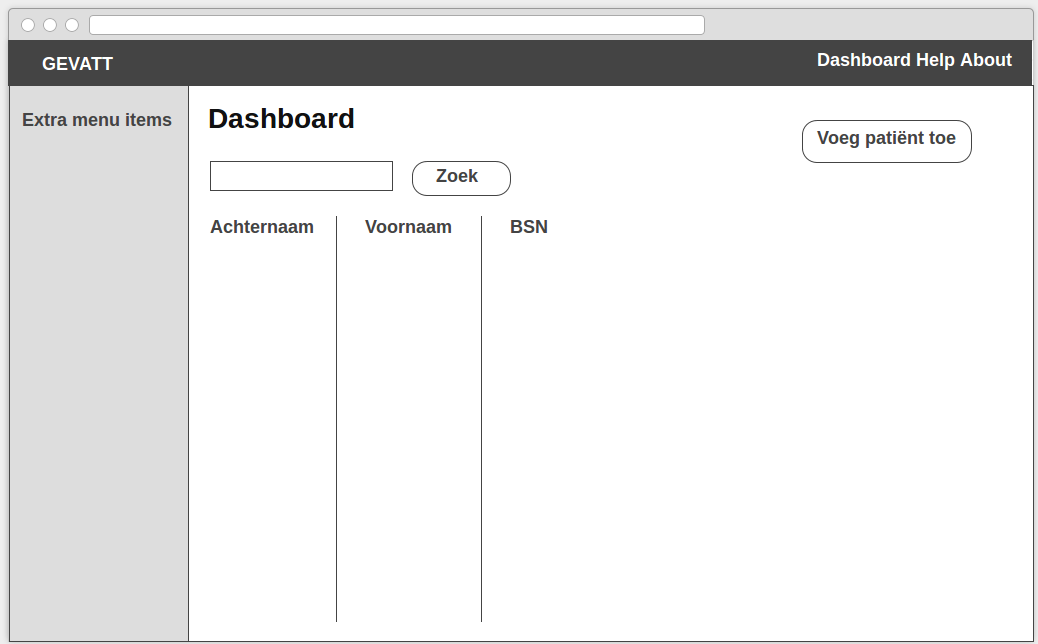
\includegraphics[scale=0.4]{select_patient.png}
\caption{A prototype of the Select Patient View}
\label{fig:selectpatientview}
\end{figure} 
In figure ~\ref{fig:selectvariationview} you see the view that you get when you click on a patient or when the VCF file of a new patient has been analysed. At this stage, you can select a variant that you want to visualise.

\begin{figure}[H]
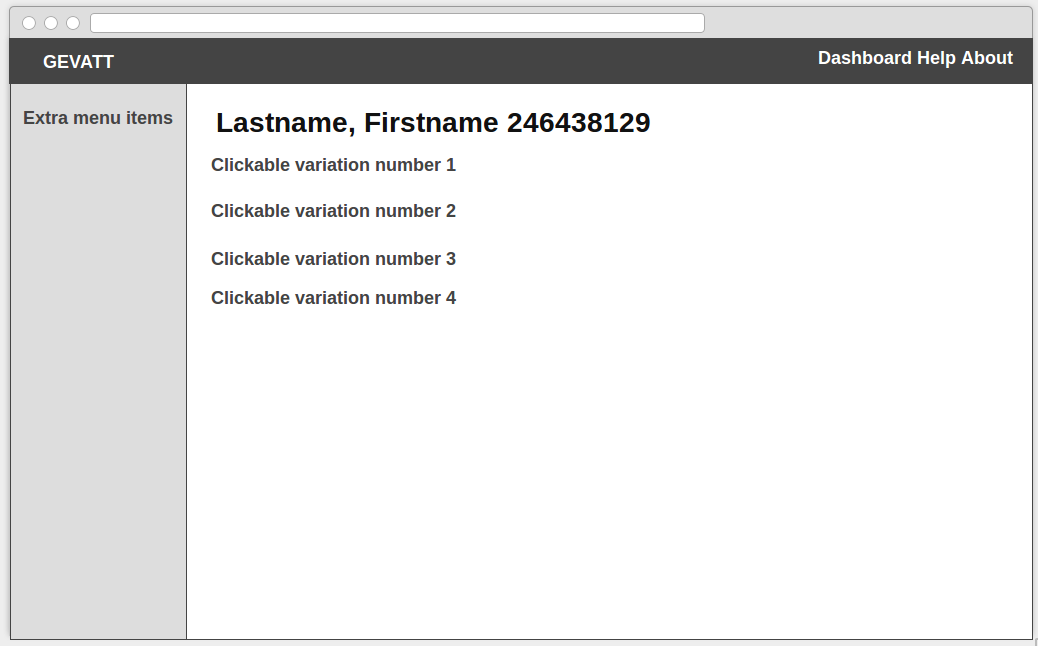
\includegraphics[scale=0.4]{select_variation.png}
\caption{A prototype of the Select Variant View}
\label{fig:selectvariationview}
\end{figure} 
In figure ~\ref{fig:lookupvariant} you see the view that you get when you click on a variant in the Select Variant View. This variant shows what type of variant you selected, what protein the base pair is a building block for, and possible diseases that could be a result of this variant.
\begin{figure}[H]
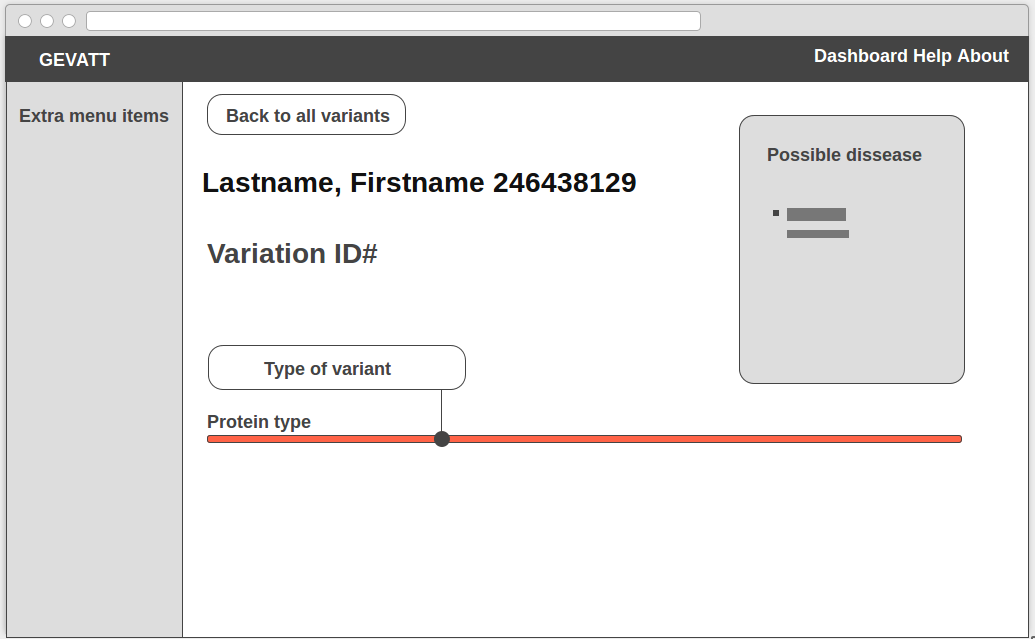
\includegraphics[scale=0.4]{lookup_variant.png}
\caption{A prototype of the Lookup Variant View}
\label{fig:lookupvariant}
\end{figure}
